\section{Territorial analysis II (Exercise 1.3)}\label{sec:territorial-II}

\paragraph{Data.}
\begin{itemize}
  \item Working inhabitants: aggregated census by IRIS RP2019~\cite{insee-census-aggregated},
  \url{https://www.insee.fr/fr/statistiques/6543200}, already aggregated to the 528 municipalities in
  \cref{sec:territorial-I}.
  \item Employees: URSSAF open data on private-sector employers and salaried employees per municipality and activity
  sector (APE)~\cite{urssaf-employment},\newline
  \href{https://open.urssaf.fr/explore/dataset/etablissements-et-effectifs-salaries-au-niveau-commune-x-ape-last/information/}{\texttt{open.urssaf.fr/explore/dataset/}\newline
  \texttt{etablissements-et-effectifs-salaries-au-niveau-commune-x-ape-last}},
  latest edition (dataset last modified on 29 May 2026, years 2006--2025), CSV export restricted to department 14,
  downloaded on 27 November 2026. We use the column \code{Effectifs salari\'es 2019}, the employees at
  \textbf{31 December 2019}: 2019 is the year of the census RP2019, so that both sources describe the same year, and it
  is also the year used in the course notebook.
  \item INSEE Code officiel g\'eographique 2026, list of changes of municipalities~\cite{insee-cog-2026},
  \url{https://www.insee.fr/fr/statistiques/fichier/8740222/v_mvt_commune_2026.csv}, to recode URSSAF to the 2021
  geography.
  \item For validation only: INSEE commuting file MOBPRO RP2019~\cite{insee-mobpro-2019},
  \url{https://www.insee.fr/fr/statistiques/6456056} (\code{FD\_MOBPRO\_2019.csv}).
\end{itemize}

\subsection{Working inhabitants per municipality (1 point)}

\begin{qa}{Make use of the aggregated census data to create a bar plot indicating the number of working inhabitants in
each municipality of the study area. Explain how you count these persons from the data.}
The bar plot is \cref{fig:working-inhabitants} (30 largest municipalities) and \cref{fig:working-inhabitants-all} in
the appendix (all 528). \textbf{We count as working inhabitants the persons aged 15 and over in the six SPCs of the
working population}, i.e.\ the sum of the columns \code{C19\_POP15P\_CS1} to \code{C19\_POP15P\_CS6} of the
aggregated census, summed from IRIS to municipality. Retirees (SPC~7) and other persons without professional activity
(SPC~8) are excluded. Calvados has 311{,}886 working inhabitants; Caen has the most (45{,}682).
\end{qa}

\paragraph{Method.}
The aggregated census does not count employed persons directly. It gives the population aged 15 and over in eight
socio-professional categories (SPC). As in the trip production model of \cref{sec:trip-production}, the
\emph{working inhabitants} of municipality $i$ are the persons aged 15 and over in the six SPCs of the working
population:
\begin{equation*}
  W^{\mathrm{res}}_i = \code{C19\_POP15P\_CS1} + \code{C19\_POP15P\_CS2} + \dots + \code{C19\_POP15P\_CS6},
\end{equation*}
i.e.\ agriculteurs exploitants; artisans, commer\c{c}ants and chefs d'entreprise; cadres and professions
intellectuelles sup\'erieures; professions interm\'ediaires; employ\'es; and ouvriers. SPC~7 (retrait\'es) and SPC~8
(autres personnes sans activit\'e professionnelle, mostly pupils, students and persons at home) are excluded. The
values per IRIS are summed to municipalities. They are weighted counts from the \emph{exploitation compl\'ementaire}
of the census, so they are not integers.
\begin{lstlisting}[style=py]
WORKING_SPC = [1, 2, 3, 4, 5, 6]        # 7 (retraites) and 8 (autres) excluded
WORKING_COLUMNS = [f"C19_POP15P_CS{k}" for k in WORKING_SPC]
df_population["working_inhabitants"] = df_population[WORKING_COLUMNS].sum(axis=1)
\end{lstlisting}

The SPC classifies persons by ``la profession (ou l'ancienne profession)''~\cite{insee-rp-definitions}. SPC 1--6
therefore count the \emph{active} population by occupation, which may include persons who are not in employment. We
measured this in the detailed census, which comes from the same exploitation as the SPC counts. We cross-tabulated
SPC and activity status (\code{TACT}) for the persons aged 15 and over of the department, with weights. Of the persons
in SPC 1--6, \textbf{88.9\,\% are employed and 11.1\,\% unemployed}. No other activity status occurs, and every
employed person is in SPC 1--6. Unemployed persons who never worked are in SPC~8. The department has 277{,}131
employed persons aged 15 and over. We keep the definition above, because the exercise asks for the aggregated census
per municipality, which has no activity status. $W^{\mathrm{res}}_i$ therefore exceeds the employed residents by
12.5\,\% at department level, and the unemployed share differs between municipalities. This difference is small
compared with the gap between the census and URSSAF, which covers only 58\,\% of the working inhabitants
(\cref{sec:territorial-II-difference}).

\begin{figure}[H]
  \centering
  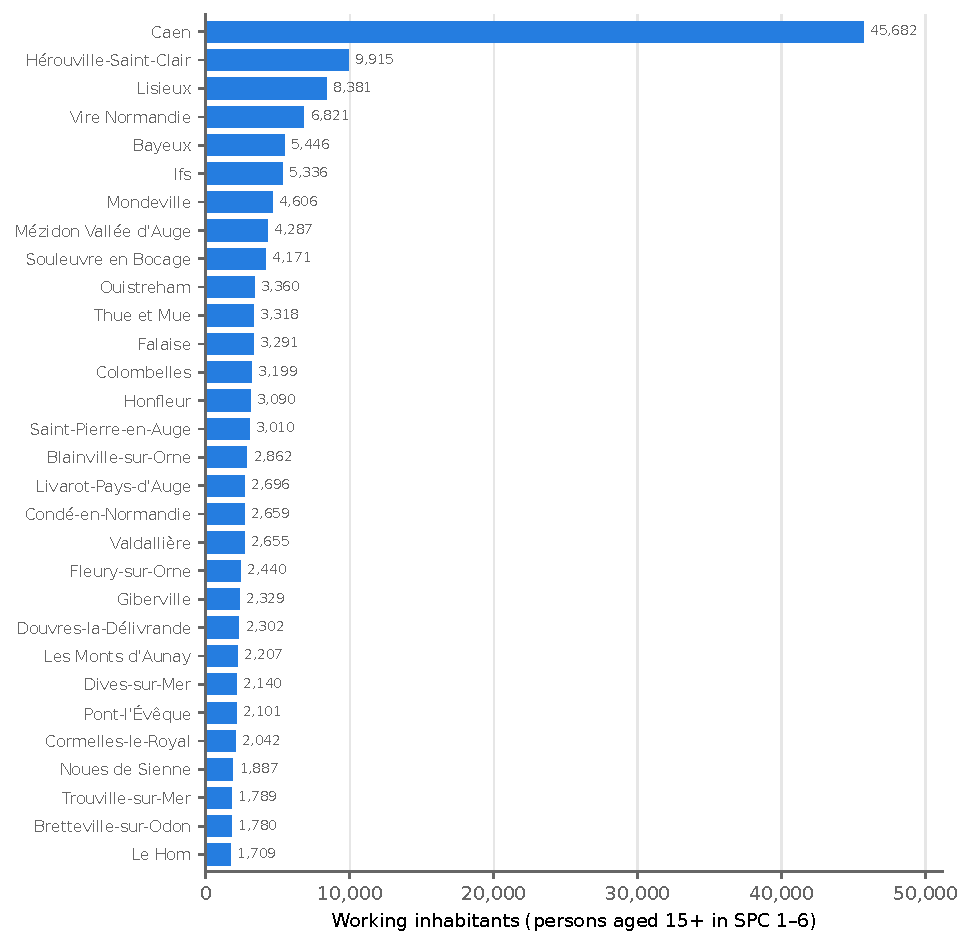
\includegraphics[width=0.85\textwidth]{working_inhabitants_top30}
  \caption{Working inhabitants (persons aged 15 and over in SPC 1--6) of the 30 municipalities of Calvados with the
  most working inhabitants. All 528 municipalities: \cref{fig:working-inhabitants-all} in the appendix. Data:
  INSEE RP2019, aggregated census by IRIS~\cite{insee-census-aggregated}.}
  \label{fig:working-inhabitants}
\end{figure}

\paragraph{Result.}
Calvados has \textbf{311{,}886 working inhabitants}: 54.1\,\% of the 576{,}234 persons aged 15 and over and 44.9\,\%
of the population. The weighted count of persons aged 15+ with SPC 1--6 in the detailed census gives the same total,
because both come from the same exploitation. \Cref{fig:working-inhabitants} shows the 30 largest municipalities.
Caen dominates with 45{,}682 working inhabitants (14.6\,\% of the department), followed by its suburb
H\'erouville-Saint-Clair (9{,}915) and the three other towns Lisieux (8{,}381), Vire Normandie (6{,}821) and Bayeux
(5{,}446). The top 30 municipalities hold 47.3\,\% of all working inhabitants. The median municipality has only 202
working inhabitants, and the smallest (Rapilly) has 10. A bar plot of all 528 municipalities, sorted, is in the
appendix (\cref{fig:working-inhabitants-all}).

\subsection{Employees per municipality (1 point)}

\begin{qa}{Make use of the URSSAF employment data to create a bar plot indicating the number of employees in each
municipality of the study area.}
The bar plot is \cref{fig:employees} (30 largest municipalities) and \cref{fig:employees-all} in the appendix
(all 528). URSSAF counts \textbf{180{,}618 private-sector salaried employees} in Calvados in 2019; Caen has the most
(35{,}246), followed by Mondeville (10{,}500).
\end{qa}

\paragraph{Method.}
The URSSAF file has one row per municipality and APE code with the number of establishments and of salaried employees
at 31 December of each year. As in the course notebook, we read \code{Code commune} as a string, keep the department
(CSV export with the filter \code{code\_departement:14}: 16{,}301 rows), and sum \code{Effectifs salari\'es 2019} over
all APE codes. Empty values are counted as 0. Of the 7{,}480 empty values, 7{,}476 belong to sectors without any
establishment in the municipality in 2019, and 4 to rows with one establishment but no count.

URSSAF uses the current geography of municipalities, while the project uses the 528 municipalities of 2021. The changes
since 1 January 2021 are taken from the INSEE list of changes of municipalities~\cite{insee-cog-2026}. Three of our
municipalities are affected:
\begin{itemize}
  \item Aurseulles changed its code from 14011 to 14581 (24 April 2024, new chef-lieu). We relabel it.
  \item Saint-Martin-de-Fontenay (14623) merged with May-sur-Orne (14408) into Saint-Martin-de-May (14408) on 1 January
  2025, with 406 employees in 2019.
  \item Gerrots (14300) merged into Victot-en-Auge (14743) on 1 January 2025, with 12 employees in 2019.
\end{itemize}
URSSAF reports only the totals of the merged municipalities. We split each total between the 2021 municipalities in
proportion to their working inhabitants. This is an assumption, and the split affects 418 employees. After recoding,
every URSSAF row is matched, and the department total is preserved. Ten small municipalities (48 to 216 inhabitants)
have no URSSAF row at all. They get \textbf{0 employees}, which means no private establishment with employees. In
total, 55 municipalities have 0 employees in 2019.
\begin{lstlisting}[style=py]
# Sum over all APE sectors per municipality (empty values count as 0)
df_urssaf = (df_urssaf_raw.groupby("Code commune")
             .agg(employees=("Effectifs salariés 2019", "sum"))
             .rename_axis("urssaf_code").reset_index())

# 2021 code -> current code, following the INSEE list of changes after 1 January 2021
changes = df_cog[
    (df_cog["DATE_EFF"] > "2021-01-01") & (df_cog["TYPECOM_AV"] == "COM") & (df_cog["TYPECOM_AP"] == "COM")
    & df_cog["COM_AV"].isin(ours) & (df_cog["COM_AV"] != df_cog["COM_AP"])
]
to_current = dict(zip(changes["COM_AV"], changes["COM_AP"]))
def current_code(code):
    while code in to_current:
        code = to_current[code]
    return code
df_match["urssaf_code"] = df_match["municipality_id"].map(current_code)

# Split the total of a merged municipality in proportion to the working inhabitants
df_match = df_match.merge(df_urssaf, on="urssaf_code", how="left", validate="m:1")
group_working = df_match.groupby("urssaf_code")["working_inhabitants"].transform("sum")
df_match["n_in_group"] = df_match.groupby("urssaf_code")["municipality_id"].transform("size")
df_match["split_share"] = np.where(df_match["n_in_group"] > 1,
                                   df_match["working_inhabitants"] / group_working, 1.0)
df_match["employees"] = (df_match["employees"] * df_match["split_share"]).fillna(0.0)   # no row -> 0
\end{lstlisting}

\emph{Scope.} URSSAF counts \emph{private-sector salaried employees at their place of work}. Not included are the
public sector (State, local authorities, public hospitals), the self-employed, and farmers and agricultural employees,
who are covered by the MSA.

\begin{figure}[H]
  \centering
  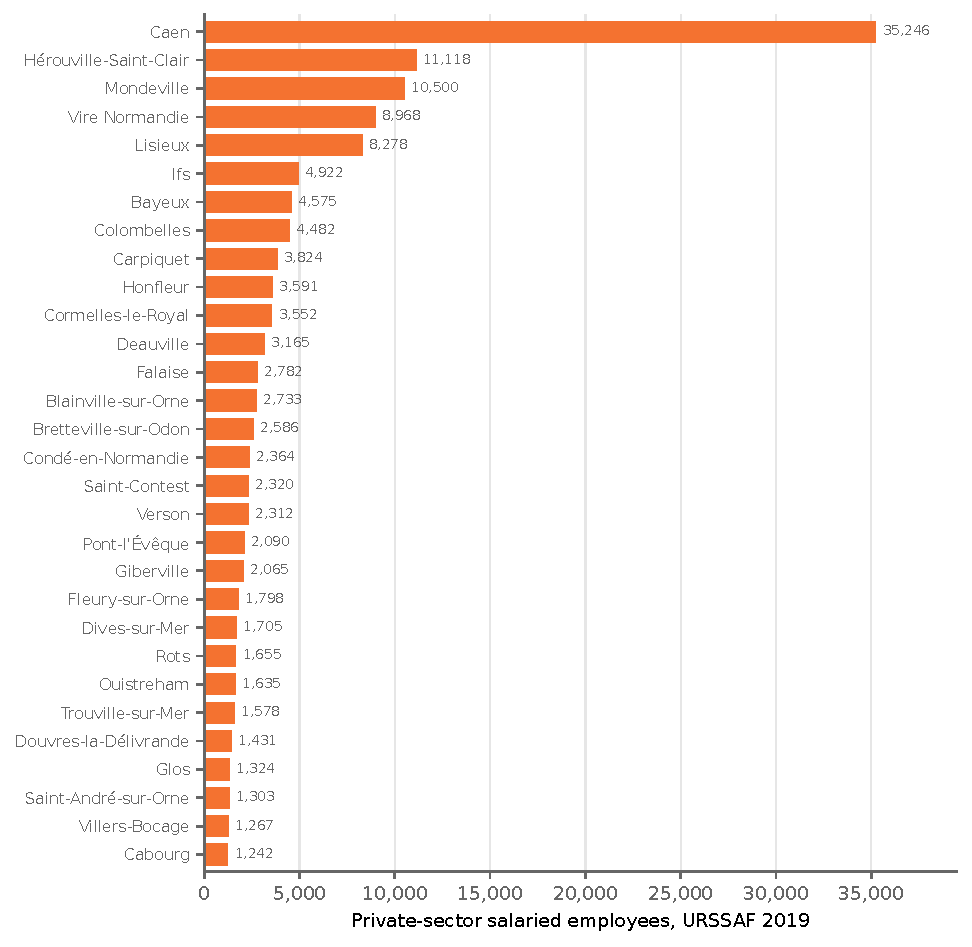
\includegraphics[width=0.85\textwidth]{employees_top30}
  \caption{Private-sector salaried employees at 31 December 2019 of the 30 municipalities of Calvados with the most
  employees, summed over all APE codes. All 528 municipalities: \cref{fig:employees-all} in the appendix. Data:
  URSSAF~\cite{urssaf-employment}.}
  \label{fig:employees}
\end{figure}

\paragraph{Result.}
URSSAF counts \textbf{180{,}618 private-sector salaried employees in Calvados in 2019}. Employment is much more
concentrated than residence (\cref{fig:employees}). Caen has 35{,}246 employees (19.5\,\% of the department), and the
top 30 municipalities hold 75.5\,\% of all employees, against 47.3\,\% of the working inhabitants. The median
municipality has 16 employees. Next to the towns, the list contains employment zones around Caen that are small as
places of residence: Mondeville (10{,}500 employees, third), Carpiquet (airport, 3{,}824), Saint-Contest, Verson and
Rots.

\subsection{Difference between working inhabitants and employees (1 point)}\label{sec:territorial-II-difference}

\begin{qa}{Make a map of the study area which, for each municipality, shows the difference between working inhabitants
and employees. Which municipality has the largest net outflow (inhabitants $-$ employees), which one the largest net
inflow of employees?}
The map is \cref{fig:net-flow-map}. \textbf{The answer to the question as asked}, i.e.\ for the raw difference
working inhabitants $-$ employees, is: the \textbf{largest net outflow is Caen} (14118, $+10{,}436$) and the
\textbf{largest net inflow is Mondeville} (14437, $-5{,}894$).

As an additional reading, we also scale the employees to the total of working inhabitants
(\cref{fig:net-flow-map-scaled}). Caen's raw outflow is an artefact of URSSAF, which misses the public-sector jobs
concentrated there, so the scaled view is more meaningful and is confirmed by the commuting data MOBPRO. In it the
largest net outflow is Souleuvre en Bocage (14061, $+3{,}032$) and the largest net inflow is Caen ($-15{,}179$).
\end{qa}

\paragraph{Method.}
For each municipality we compute $\Delta_i = W^{\mathrm{res}}_i - E_i$, working inhabitants minus employees. A
positive value means more working residents than jobs, i.e.\ a \emph{net outflow} of commuters. A negative value means
a \emph{net inflow} of employees. The map (\cref{fig:net-flow-map}) uses a diverging colour scale centred at 0, with
blue for inflow and red for outflow, and symmetric limits $\pm\max_i|\Delta_i|$. Caen alone reaches $\pm 10^4$, so
the scale is a symmetric logarithm: linear within $\pm 100$ persons and logarithmic beyond.

\paragraph{Comparability.}
The two sources do not measure the same thing. The census counts all working residents, at their place of residence:
the public sector, the self-employed and farmers, and unemployed persons with a former occupation (11.1\,\% of SPC
1--6). URSSAF counts private salaried jobs, at the place of work. The totals are 311{,}886 working inhabitants and 180{,}618
employees: URSSAF covers only \textbf{58\,\%} of the census count (ratio 0.579). The raw difference is therefore
positive in 505 of the 528 municipalities and sums to $+131{,}268$. As an additional view, we scale the employees to
the total of working inhabitants, $\tilde E_i = E_i \cdot \sum_k W^{\mathrm{res}}_k / \sum_k E_k$ (factor 1.727). The
scaled difference $\tilde\Delta_i = W^{\mathrm{res}}_i - \tilde E_i$ sums to 0 and shows the relative pattern
(\cref{fig:net-flow-map-scaled}). This is also how employment enters the trip attraction in \cref{sec:trip-attraction}:
arriving trips are proportional to employment.
\begin{lstlisting}[style=py]
df_population["difference"] = df_population["working_inhabitants"] - df_population["employees"]
scale_factor = working_total / employees_total                     # 1.727
df_population["difference_scaled"] = (df_population["working_inhabitants"]
                                      - scale_factor * df_population["employees"])
outflow = df_population.nlargest(1, "difference")     # largest net outflow
inflow = df_population.nsmallest(1, "difference")     # largest net inflow
\end{lstlisting}

\begin{figure}[H]
  \centering
  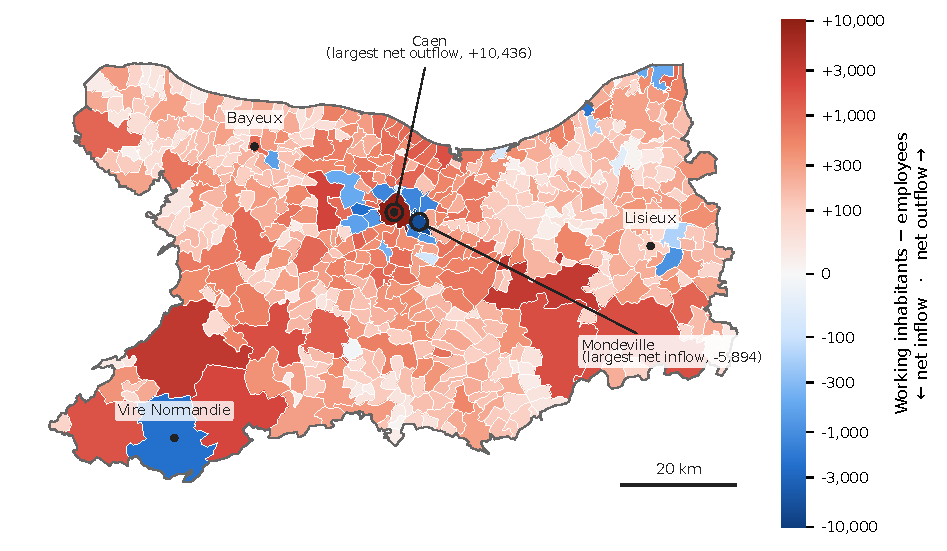
\includegraphics[width=\textwidth]{inhabitants_minus_employees_map}
  \caption{Working inhabitants (census RP2019, SPC 1--6) minus private-sector salaried employees (URSSAF 2019) per
  municipality. Red: net outflow; blue: net inflow. Symmetric logarithmic colour scale, linear within $\pm 100$.
  Circles: largest net outflow and largest net inflow. Data: INSEE~\cite{insee-census-aggregated},
  URSSAF~\cite{urssaf-employment}, IGN CONTOURS-IRIS 2021~\cite{ign-contours-iris}; Lambert-93.}
  \label{fig:net-flow-map}
\end{figure}

\paragraph{Result.}
\begin{itemize}
  \item \textbf{Largest net outflow: Caen} (14118): 45{,}682 working inhabitants, 35{,}246 employees, difference
  $+10{,}436$.
  \item \textbf{Largest net inflow: Mondeville} (14437): 4{,}606 working inhabitants, 10{,}500 employees, difference
  $-5{,}894$.
\end{itemize}
The result for Caen is an effect of the definitions. Caen is the main employment centre of the department, but it
concentrates the public-sector jobs that URSSAF does not count (university, regional hospital, administrations).
Its working residents are therefore compared with its private jobs only. Mondeville, with commercial and industrial zones
east of Caen, has more than twice as many private jobs as working residents.

Only 23 municipalities have a net inflow in the raw view: the employment zones around Caen (Mondeville, Carpiquet,
Cormelles-le-Royal, H\'erouville-Saint-Clair, Colombelles), Vire Normandie, and the resort Deauville
(\cref{tab:net-flow-top5}). The largest outflows are Caen and large rural \emph{communes nouvelles} with few private
jobs (Souleuvre en Bocage, M\'ezidon Vall\'ee d'Auge, Thue et Mue, Valdalli\`ere).

\begin{table}[H]
  \centering
  \caption{The five municipalities with the largest net outflow and the five with the largest net inflow, raw
  difference $\Delta_i$ and scaled difference $\tilde\Delta_i$ (employees $\times\,1.727$). Bold: the answer per view.}
  \label{tab:net-flow-top5}
  \small
  \setlength{\tabcolsep}{4pt}
  \begin{tabular}{@{}llrrr@{\hspace{1.5em}}llr@{}}
    \toprule
    \multicolumn{5}{c}{Raw: $\Delta_i = W^{\mathrm{res}}_i - E_i$} & \multicolumn{3}{c}{Scaled: $\tilde\Delta_i$} \\
    \cmidrule(r{1.5em}){1-5}\cmidrule{6-8}
    Code & Municipality & $W^{\mathrm{res}}_i$ & $E_i$ & $\Delta_i$ & Code & Municipality & $\tilde\Delta_i$ \\
    \midrule
    \multicolumn{8}{@{}l}{\emph{Largest net outflow}} \\
    14118 & \textbf{Caen} & 45{,}682 & 35{,}246 & $+$10{,}436 & 14061 & \textbf{Souleuvre en Bocage} & $+$3{,}032 \\
    14061 & Souleuvre en Bocage & 4{,}171 & 660 & $+$3{,}511 & 14431 & M\'ezidon Vall\'ee d'Auge & $+$2{,}814 \\
    14431 & M\'ezidon Vall\'ee d'Auge & 4{,}287 & 853 & $+$3{,}434 & 14726 & Valdalli\`ere & $+$1{,}805 \\
    14098 & Thue et Mue & 3{,}318 & 907 & $+$2{,}411 & 14098 & Thue et Mue & $+$1{,}752 \\
    14726 & Valdalli\`ere & 2{,}655 & 492 & $+$2{,}163 & 14027 & Les Monts d'Aunay & $+$1{,}561 \\
    \midrule
    \multicolumn{8}{@{}l}{\emph{Largest net inflow}} \\
    14437 & \textbf{Mondeville} & 4{,}606 & 10{,}500 & $-$5{,}894 & 14118 & \textbf{Caen} & $-$15{,}179 \\
    14137 & Carpiquet & 1{,}495 & 3{,}824 & $-$2{,}329 & 14437 & Mondeville & $-$13{,}525 \\
    14762 & Vire Normandie & 6{,}821 & 8{,}968 & $-$2{,}147 & 14327 & H\'erouville-Saint-Clair & $-$9{,}283 \\
    14220 & Deauville & 1{,}283 & 3{,}165 & $-$1{,}882 & 14762 & Vire Normandie & $-$8{,}665 \\
    14181 & Cormelles-le-Royal & 2{,}042 & 3{,}552 & $-$1{,}510 & 14366 & Lisieux & $-$5{,}913 \\
    \bottomrule
  \end{tabular}
\end{table}

\begin{figure}[H]
  \centering
  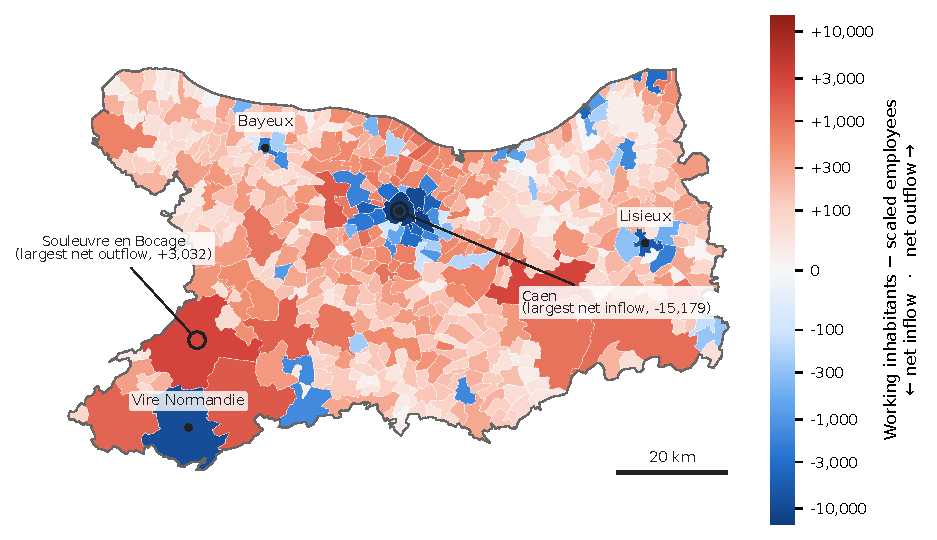
\includegraphics[width=\textwidth]{inhabitants_minus_employees_scaled_map}
  \caption{Working inhabitants minus \emph{scaled} employees, $\tilde\Delta_i = W^{\mathrm{res}}_i - 1.727\,E_i$
  (employees scaled to the total of working inhabitants). Same colour scale as \cref{fig:net-flow-map}, with
  symmetric limits $\pm 15{,}179$. Data as in \cref{fig:net-flow-map}.}
  \label{fig:net-flow-map-scaled}
\end{figure}

\paragraph{Scaled view.}
After scaling, the picture matches the urban structure (\cref{fig:net-flow-map-scaled}). \textbf{Caen becomes the
largest net inflow} ($-15{,}179$), followed by Mondeville, H\'erouville-Saint-Clair, Vire Normandie and Lisieux.
\textbf{The largest net outflow is Souleuvre en Bocage} (14061; $+3{,}032$), a rural commune nouvelle north-east of Vire.
36 municipalities change side, all from outflow to inflow. Together they hold 33.7\,\% of the working inhabitants.
They include Caen, Lisieux, Bayeux, Ifs, Falaise, Condé-en-Normandie and Pont-l'\'Ev\^eque, i.e.\ the towns whose
private employment is close to their number of working residents. The number of inflow municipalities rises from 23
to 59. The scaled view assumes that the jobs URSSAF does not count are distributed like private salaried jobs. It is
not exact either, but it is the more meaningful answer to the question. It is also the assumption used for the
trip attraction in \cref{sec:trip-attraction}.

\subsection{Validation with commuting data}\label{sec:territorial-II-mobpro}

\paragraph{Data.}
INSEE's commuting file MOBPRO~\cite{insee-mobpro-2019} gives, for every employed person of the census RP2019, the
municipality of residence (\code{COMMUNE}) and the municipality of work (\code{DCLT}), with the weight \code{IPONDI}.
Unlike URSSAF, it covers \emph{all} jobs, including the public sector, the self-employed and farmers. It uses the same
year (2019) and the same geography (2021) as our census. It is therefore the real-data reference for the net commuting
balance of each municipality. As in the course notebook, we read \code{COMMUNE}, \code{ARM}, \code{DCLT},
\code{IPONDI} and \code{TRANS} in chunks. We keep every person who lives \emph{or} works in Calvados, so that commuters
from and to other departments are included. All department codes in the file are among our 528 municipalities. Every
municipality has employed residents, and 7 small municipalities have no job. For each municipality $i$ we compute
the employed residents $R_i$ (living in $i$), the jobs $J_i$ (working in $i$, wherever the person lives) and the net
balance $N_i = R_i - J_i$, with the same sign convention as $\Delta_i$. This is a validation only: the answers above
remain those based on the census and URSSAF, as the exercise asks.

\begin{table}[H]
  \centering
  \caption{Department totals of Calvados, 2019. The census counts are at the place of residence, the job counts at
  the place of work. Data: INSEE~\cite{insee-census-aggregated,insee-census-detailed,insee-mobpro-2019},
  URSSAF~\cite{urssaf-employment}.}
  \label{tab:mobpro-totals}
  \begin{tabular}{@{}llr@{}}
    \toprule
    Quantity & Counted at & Persons \\
    \midrule
    Census: working inhabitants $W^{\mathrm{res}}$ (aged 15+, SPC 1--6) & residence & 311{,}886 \\
    Census: employed persons aged 15+ (\code{TACT} $=$ 11) & residence & 277{,}131 \\
    MOBPRO: employed residents $R$ & residence & 277{,}131 \\
    MOBPRO: jobs located in Calvados $J$ & workplace & 275{,}908 \\
    URSSAF: private-sector salaried employees $E$ & workplace & 180{,}618 \\
    \bottomrule
  \end{tabular}
\end{table}

\paragraph{Totals.}
MOBPRO counts exactly the employed persons of the detailed census (\cref{tab:mobpro-totals}), because both are the
same census records with the same weights. The working inhabitants are 12.5\,\% higher, as measured in
\cref{sec:territorial-II} with \code{TACT}. Per municipality, $W^{\mathrm{res}}_i$ and $R_i$ correlate at 0.9997, and
the median ratio is 1.09. The SPC definition therefore shifts the level but hardly changes the pattern. 30.0\,\% of
the employed residents work in their own municipality. 21{,}882 residents (7.9\,\%) work outside Calvados, mainly in
Manche, Orne, Seine-Maritime, Eure and Paris. 20{,}659 persons living outside work in Calvados, mainly from Manche,
Eure and Orne. Calvados is therefore almost balanced: 1{,}223 more residents commute out than workers commute in.

\paragraph{Jobs not counted by URSSAF.}
URSSAF covers 65.5\,\% of the 275{,}908 jobs located in Calvados. Of the 95{,}290 jobs that URSSAF misses, 40\,\%
are in Caen, which has 73{,}271 jobs but only 35{,}246 URSSAF employees (coverage 48\,\%: university, regional
hospital, administrations). Next come Lisieux (5{,}215 jobs missed), Bayeux (3{,}817), Falaise and Vire Normandie,
towns with hospitals, schools and sub-prefectures. This confirms the explanation given for Caen in
\cref{sec:territorial-II-difference}. In 38 municipalities, URSSAF has \emph{more} employees than MOBPRO has jobs,
mostly commercial and industrial zones around Caen (Mondeville $+666$, Bretteville-sur-Odon $+607$). URSSAF counts job
positions at 31 December: persons with two jobs count twice, and temporary workers count where the agency is. MOBPRO
counts persons at the place of their main job.

\begin{figure}[H]
  \centering
  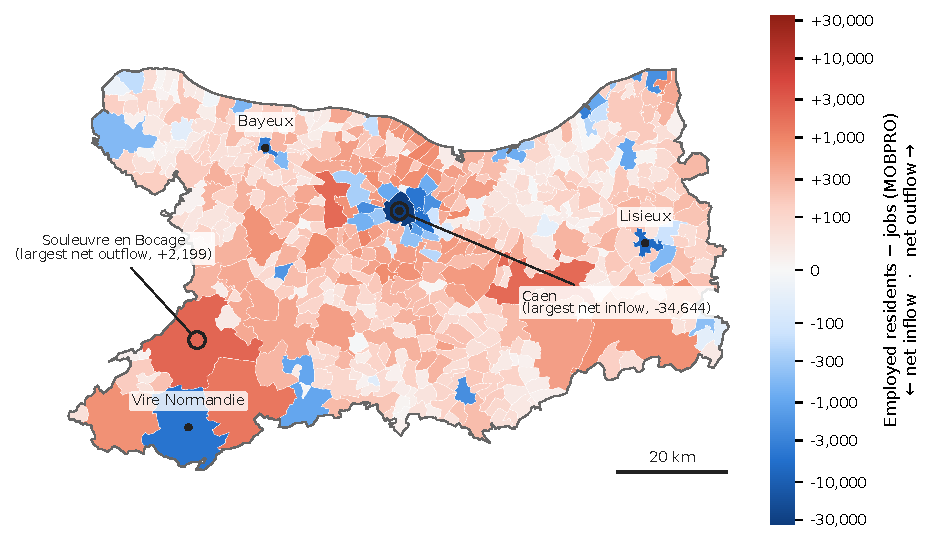
\includegraphics[width=\textwidth]{net_commuting_mobpro_map}
  \caption{Net commuting according to MOBPRO, employed residents minus jobs, per municipality. Red: net outflow;
  blue: net inflow. Same colour scale as \cref{fig:net-flow-map} (symmetric logarithm, linear within $\pm 100$), with
  symmetric limits $\pm 34{,}644$. Data: INSEE MOBPRO RP2019~\cite{insee-mobpro-2019}, IGN CONTOURS-IRIS
  2021~\cite{ign-contours-iris}; Lambert-93.}
  \label{fig:net-commuting-mobpro}
\end{figure}

\begin{figure}[H]
  \centering
  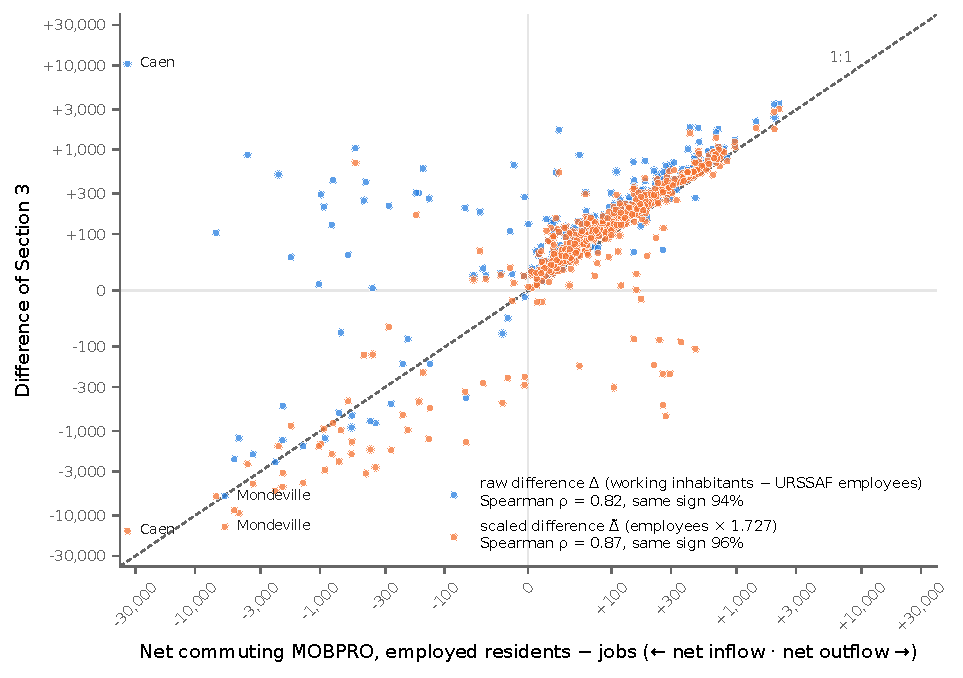
\includegraphics[width=0.9\textwidth]{difference_vs_mobpro}
  \caption{Raw difference $\Delta_i$ (blue) and scaled difference $\tilde\Delta_i$ (orange) of each municipality
  against the net commuting $N_i$ of MOBPRO. Both axes use a symmetric logarithm, linear within $\pm 100$. Points on
  the dashed line agree exactly. Data: as in \cref{fig:net-flow-map,fig:net-commuting-mobpro}.}
  \label{fig:difference-vs-mobpro}
\end{figure}

\paragraph{Net commuting.}
According to MOBPRO (\cref{fig:net-commuting-mobpro}), the \textbf{largest net inflow is Caen} (14118): 38{,}627
employed residents, 73{,}271 jobs, $N = -34{,}644$. Next come Lisieux ($-6{,}749$), Mondeville ($-5{,}785$), Vire
Normandie ($-4{,}837$) and H\'erouville-Saint-Clair ($-4{,}465$). The \textbf{largest net outflow is Souleuvre en
Bocage} (14061; $+2{,}199$), followed by Thue et Mue ($+2{,}020$) and M\'ezidon Vall\'ee d'Auge ($+2{,}009$).
54 municipalities have a net inflow (raw view: 23, scaled view: 59). Both extremes are the answers of the
\emph{scaled} view, while the raw view gives Caen the wrong sign. \Cref{tab:mobpro-agreement} and
\cref{fig:difference-vs-mobpro} show that \textbf{the scaled view is closer to reality} on every measure. Its
magnitudes are still wrong where the mix of jobs is unusual. It finds less than half of Caen's real inflow
($-15{,}179$ against $-34{,}644$) and more than twice the inflow of Mondeville ($-13{,}525$ against $-5{,}785$).
For Mondeville the raw value ($-5{,}894$) is almost exact. Scaling assumes that every municipality has the
department's share of private jobs, which does not hold for an administrative centre or a private employment zone.

\begin{table}[H]
  \centering
  \caption{Agreement of the raw difference $\Delta_i$ and the scaled difference $\tilde\Delta_i$ with the net
  commuting $N_i$ of MOBPRO, over the 528 municipalities.}
  \label{tab:mobpro-agreement}
  \begin{tabular}{@{}lrr@{}}
    \toprule
    Measure & Raw $\Delta_i$ & Scaled $\tilde\Delta_i$ \\
    \midrule
    Pearson correlation & $-0.40$ & 0.78 \\
    Pearson correlation without Caen & 0.68 & 0.90 \\
    Spearman rank correlation & 0.82 & 0.87 \\
    Municipalities with the same sign as $N_i$ & 94.1\,\% & 95.6\,\% \\
    Mean absolute deviation from $N_i$ (persons) & 258 & 208 \\
    \bottomrule
  \end{tabular}
\end{table}

The table of origin--destination flows with both ends in Calvados (255{,}249 persons in 9{,}866 pairs of
municipalities, summed over the modes) is saved for the validation of the gravity model in \cref{sec:trip-distribution}.

\paragraph{Problems encountered.}
\begin{itemize}
  \item \emph{Definition of working inhabitants.} The aggregated census has no count of employed persons, and SPC
  1--6 also classify persons by a former occupation. Measured in the detailed census (SPC $\times$ \code{TACT}),
  88.9\,\% of the persons in SPC 1--6 are employed and 11.1\,\% unemployed, so $W^{\mathrm{res}}_i$ exceeds the
  employed residents by 12.5\,\%. This is small compared with the gap between census and URSSAF: URSSAF counts 58\,\%
  of the working inhabitants and still only 65\,\% of the 277{,}131 employed persons.
  \item \emph{Different municipality geography.} URSSAF uses the current geography, the project that of 2021: one
  change of code (Aurseulles) and two mergers on 1 January 2025 (Saint-Martin-de-Fontenay into Saint-Martin-de-May,
  Gerrots into Victot-en-Auge). Codes were recoded with the INSEE list of changes~\cite{insee-cog-2026}. The merged
  totals (418 employees) were split in proportion to working inhabitants.
  \item \emph{Missing municipalities and empty values.} Ten small municipalities have no URSSAF row and get 0
  employees. The empty 2019 values (7{,}480 rows) are sectors without an establishment in that year and are counted
  as 0.
  \item \emph{Different definitions of the two sources.} Private salaried jobs at the workplace (URSSAF) cover only
  58\,\% of the working residents (census). Without scaling, Caen appears as the largest net outflow, which is an
  effect of the missing public-sector jobs. We therefore report both the raw and the scaled difference.
\end{itemize}
